%% This is an example first chapter.  You should put chapter/appendix that you
%% write into a separate file, and add a line \include{yourfilename} to
%% main.tex, where `yourfilename.tex' is the name of the chapter/appendix file.
%% You can process specific files by typing their names in at the
%% \files=
%% prompt when you run the file main.tex through LaTeX.
\section{Geometry}
\label{sec:geom}

The intersection of convex objects is a matter well studied for multiple
subjects. In our case, it is interesting to know some properties about
the intersection of disks, those ones being convex objects.

A set $S$ is convex if:
$$\forall p,q \in S\  \forall \lambda \in [0,1]: (1-\lambda)p + \lambda q \in S$$

\subsection{Stabbing}
A \textit{stabbing} is a point that traverses a set of intersecting objects. A lot of
research has been done \cite{schlipf2013stabbing} on the minimal amount of stabbings to
cover every object in a set. Stabbings can also be done with more complex structures
than points, in that case we are talking about \textit{coverings}.

\begin{theorem}[Helly]
  Given a set $Q$ of objects in $\mathbb{R}^d$, if for each subset of $Q$ of
  size $d+1$ their intersection is non empty, then $\bigcap_{q \in Q} \neq
  \varnothing$. \cite{Helly1923175}
\end{theorem}

\begin{theorem}
  The problem that for a set of $n$ disks whether there exists a regular n-gon
  whose vertices stab every disk of the set can be decided in $O(n^{10.5} / \sqrt{\log(n)})$ \cite{schlipf2013stabbing}
\end{theorem}

\subsection{Coin graphs}

Penny graphs can be defined as disk graphs where the disks can just touch each
other without overlapping. A famous theorem is derived from this class of graphs:
the circle packing theorem.

\begin{theorem}[Circle packing theorem]
  The circle packing theorem states that for every simple connected planar graph
  $G$ is a penny graph. \cite{doi:10.1137/0406017}
\end{theorem}

\begin{corollary}
  Planar graphs $\subseteq$ disk graphs \cite{spinradEfficientGraphRepresentations2012}.
\end{corollary}

\begin{figure}
\centering
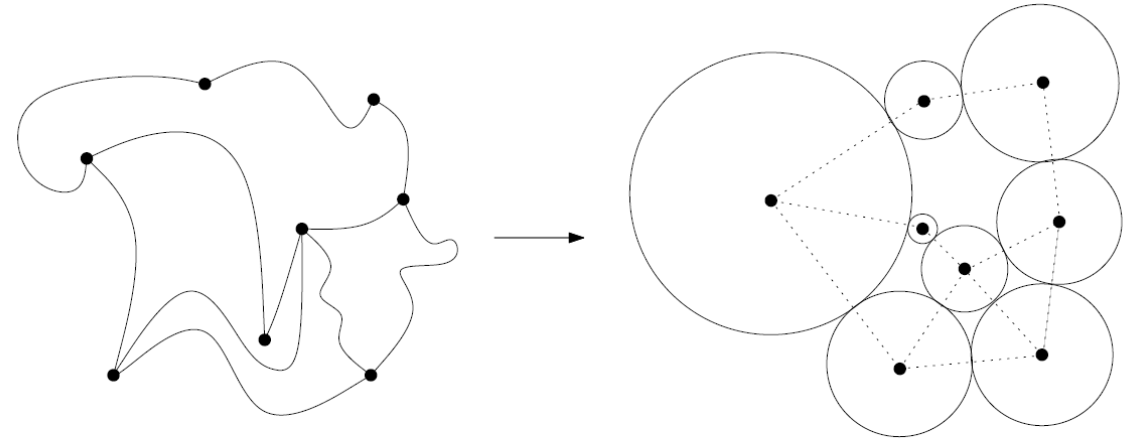
\includegraphics[width=1.0\textwidth]{res/circle_packing}
\caption{Circle packing of a planar graph. \cite{nachmiasPlanarMapsRandom2016}}
\label{fig:circle}
\end{figure}
